%----------------------------------------------------------------------------------------
%	PACKAGES AND DOCUMENT CONFIGURATIONS
%----------------------------------------------------------------------------------------

\documentclass{article}

\usepackage{graphicx} % Required for the inclusion of images
\usepackage{natbib} % Required to change bibliography style to ABB
\usepackage{amsmath} % Required for some math elements

\usepackage{times}

\newcommand{\newpar}{\smallskip\noindent} %command to create new paragraph with no ident.
%----------------------------------------------------------------------------------------
%	DOCUMENT INFORMATION
%----------------------------------------------------------------------------------------

\title{OCCT: One Class Clustering Tree\\ Implementation for Weka} % Title

\author{\textsc{Vitali Sepetnitsky, Maor Tal}} % Author name

\date{\today} % Date for the report

\begin{document}

\maketitle % Insert the title, author and date

\begin{center}
Instructor: Dr. Asaf Shabtai % Instructor/supervisor
\end{center}


%----------------------------------------------------------------------------------------
%	SECTION 1 - Introduction
%----------------------------------------------------------------------------------------

\section{Introduction}
Data linkage is the task of identifying different entries (i.e., data items) that refer to the same
entity across different data sources \cite{damaging2011}, \cite{kamra2008detecting}. Record linkage refers to the task of joining datasets
that do not share a common identifier (i.e., a foreign key). 

\subsection{OCCT}
The two common types of data linkage are: 
\begin{itemize}
  \item \emph{one-to-one} data linkage in which the goal is to associate
an entity from one dataset with a single matching entity from the another dataset.
  \item \emph{one-to-many} where the goal is to associate an entity from the first
   dataset to a group of matching entities from the other dataset. 
\end{itemize}
\newpar{OCCT} (One-Class Clustering Tree) is a novel data linkage method, presented in \cite{dror2011thesis} and \cite{dror2014occt},
which is capable of performing one-to-many data linkage between entities of same or different
types. The tree is built such that it is easy to transform it into association rules.

One of the major advantages of OCCT compared to other data linkage methods, is using the
one-class approach. This means that it needs only examples of matching pairs in order to learn
and build the model. This feature is important since in many domains it is difficult to obtain
nonmatching examples (e.g. the fraud detection domain).

Building the tree requires deciding which attribute should be selected at each level. There are
four different “splitting criteria” proposed by the authors in \cite{dror2014occt}, along with two pre-pruning process,
to stop expanding branches that does not improve the accuracy of the model.

Once the construction of the tree is completed, a set of probabilistic models are induced for each
of the leafs of the tree.
Each model is deriving the probability of a value of a given attribute from table ($T_{B}$) that
is most likely to be linked with a record from the first table ($T_{A}$).

\subsection{Weka}
Weka (Waikato Environment for Knowledge Analysis) is a suite of machine learning software
which contains a collection of algorithms and visualization tools for data analysis and machine
learning, along with graphical user interfaces for easy access to its functionality. Weka is
free software available under the GNU General Public License.
It is written in Java and developed at the University of Waikato, New Zealand. Weka is also well-suited 
for developing new machine learning schemes.

%----------------------------------------------------------------------------------------
%	SECTION 2 - Motivation, Project Goals
%----------------------------------------------------------------------------------------
\section{Motivation}
OCCT was evaluated by the authors in \cite{dror2011thesis} and \cite{dror2014occt} as a part of a detection system framework
designed for detecting potential data leakage/misuse. The detection system was
designed to incorporate multiple detectors as plug-ins, where each detector implements a
different detection algorithm, such as OCCT.

The original implementation suffered from many drawbacks, especially it was designed for a
specific domain and did not use any common interfaces which are used in Weka. This made it impossible to
be used by other researchers in order to perform more extensive evaluation and research on OCCT.
In addition evaluating OCCT versus other data linkage algorithms which are already implemented within Weka
was a tedious task.

Our project goal is to implement OCCT, using Weka common API for machine learning
algorithms, and provide basic evaluation of OCCT using our implementation. We intend to add
OCCT as one of the classifiers in Weka UI and make it available to researchers who wishes to further
evaluate OCCT.

%----------------------------------------------------------------------------------------
%	SECTION 3 - Code Structure
%----------------------------------------------------------------------------------------
\section{Code Structure}
The code was carefully designed in order to be flexible for future extensions and also be as readable as possible.
Its implementation is based on the J48, which is an open source Java implementation of the C4.5 algorithm in Weka.   

\clearpage
\subsection{Main structure}
\begin{figure}[!h]
    \centering
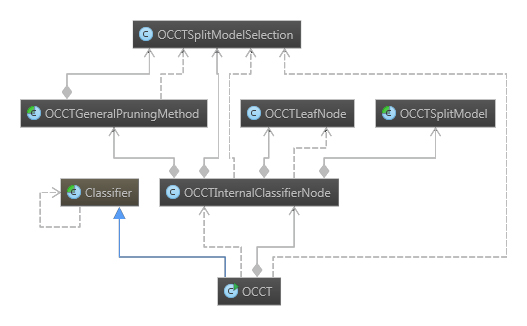
\includegraphics[width=1\textwidth]{Figures/MainStructure}
    \caption{Main OCCT structure}
    \label{fig:mainstr}
\end{figure}










%----------------------------------------------------------------------------------------
\bibliographystyle{abbrv}
\bibliography{refFile}

\end{document}